\section{Анализ производительности}

Мы реализовали три алгоритма на языке программирования \OCaml\footnote{\url{https://github.com/ProgMiner/rational-unification}}:
\begin{itemize}
    \item \texttt{robinson}~--- алгоритм Робинсона с <<треугольными>> подстановками~\cite{baader2001unification};
    \item \texttt{rational}~--- наш алгоритм, описанный выше;
    \item \texttt{huet}~--- алгоритм Юэ~\cite{huet1976resolution} на основе реализации в SWI-Prolog\footnote{\url{https://github.com/SWI-Prolog/swipl/blob/45e83178379f0fd6f918bd294bb361f3db7bf1d7/src/pl-prims.c\#L71}}.
\end{itemize}

Все три алгоритма были реализованы в двух вариантах: эфемерном (с изменяемыми переменными) и персистентном. Дополнительно были реализованы эфемерные варианты алгоритмов со сжатием путей. Для справедливого сравнения все реализации выполнены с наиболее подходящими структурами данных и оптимизированы насколько это было возможно.

Для тестирования использовались <<трассы унификации>>. Каждая трасса представляет собой список уравнений, где каждое уравнение задано парой термов. Всего было подготовлено три набора тестов:
\begin{itemize}
    \item \texttt{JGS}~--- собраны автоматически из тестов <<Java Generic Solver>>~\cite{lozov2023relational} (9 тестов, 1448 трасс);
    \item \texttt{Lama}~--- собраны автоматически из тестов <<Lama type checker>>~\cite{domoratskiy2024relational} (66 трасс, по одной на тест);
    \item \texttt{synth}~--- синтетические тесты, сгенерированны вручную (66 трасс, по 11 на тест).
\end{itemize}

Мы считаем наборы тестов \texttt{JGS} и \texttt{Lama} близкими к прикладным задачам унификации <<из реального мира>>. Для выполнения трасс из набора \texttt{JGS} достаточно классической унификации (конечных термов), тогда как некоторые трассы из набора \texttt{Lama} требуют поддержки рациональной унификации.

Синтетические тесты были подобраны эмпирически для нагрузочного тестирования алгоритмов. Каждый из перечисленных тестов параметризован числом $n = 0, 10, ..., 100$:
\begin{itemize}
    \item \texttt{full}~--- уравнивает два полных двоичных дерева глубины $n$ ($T_i, U_i \in \V$):
    \begin{equation*}
        \left\{
        \begin{array}{c@{{}={}}ll}
            T_0 & x, & x \in \V, \\
            U_0 & a, & a^0 \in \C, \\
            T_i & f\,(T_{i-1}, T_{i-1}), & i = 1, 2, \dots, n, \\
            U_i & f\,(U_{i-1}, U_{i-1}), & i = 1, 2, \dots, n, \\
            T_n & U_n. \\
        \end{array}
        \right.
    \end{equation*}
    \item \texttt{left\_right}~--- уравнивает <<левостороннее>> и <<правостороннее>> двоичные деревья глубины $n$ ($T_i, U_i \in \V$):
    \begin{equation*}
        \left\{
        \begin{array}{c@{{}={}}ll}
            T_0 & x, \\
            U_0 & x, \\
            T_i & f\,(T_{i-1}, x), & i = 1, 2, \dots, n, \\
            U_i & f\,(x, U_{i-1}), & i = 1, 2, \dots, n, \\
            T_n & U_n. \\
        \end{array}
        \right.
    \end{equation*}
    \item $\texttt{loops}_1$~--- уравнивает $n$ <<петель>> друг с другом:
    \begin{equation*}
        \left\{
        \begin{array}{c@{{}={}}ll}
            x_i & f\,(x_i), & i = 1, 2, \dots, n, \\
            x_0 & x_i, & i = 1, 2, \dots, n. \\
        \end{array}
        \right.
    \end{equation*}
    \item $\texttt{loops}_2$ --- как предыдущий, но с $x_i = x_0$ вместо $x_0 = x_i$.
    \item $\texttt{loops}_3$ --- как $\texttt{loops}_1$, но с $x_{i-1} = x_i$ вместо $x_0 = x_i$.
    \item $\texttt{loops}_4$ --- как предыдущий, но с $x_i = x_{i-1}$ вместо $x_{i-1} = x_i$.
\end{itemize}

Все синтетические тесты, кроме \texttt{full}, требуют поддержки рациональной унификации. Тем не менее, тест \texttt{full} затрачивает экспоненциальное количество времени и памяти при запуске на алгоритме Робинсона. По этой причине, синтетические тесты использовались только для сравнения алгоритмов рациональной унификации между собой.

Замеры проводились на компьютере под управлением ОС Alpine Linux с изоляцией одного ядра процессора (13th Gen Intel® Core™ i7-1360P) и прикреплением тестирующего процесса к выделенному ядру\footnote{\url{https://github.com/ProgMiner/bench-linux}}. Все промежуточные результаты замеров приведены в упомянутом ранее репозитории и могут быть воспроизведены.

Основные результаты сравнения:
\begin{itemize}
    \item Наш алгоритм работает настолько же быстро, насколько и классический алгоритм Робинсона в <<реальных>> сценариях использования, что продемонстрировано на \autoref{fig:baseline}. Приведённые графики отражают время работы алгоритмов рациональной унификации по отношению ко времени работы алгоритма Робинсона. В частности, на графиках видно, что наш алгоритм в обоих случаях держится вблизи главной диагонали.
    \item Несмотря на то, что алгоритм Юэ работает быстрее в эфемерной реализации, он деградирует будучи реализованным персистентно~--- это отражено как на \autoref{fig:baseline}, так и на \autoref{fig:Lama}. Более того, \autoref{fig:synth-ephemeral} и \autoref{fig:synth-persistent} также демонстрируют, что в некоторых случаях алгоритм Юэ начинает работать значительно медленнее даже в эфемерной реализации, а также, что время его работы зависит от порядка сторон уравнений (разница между $\texttt{loops}_1$ и $\texttt{loops}_2$).
\end{itemize}

\begin{figure}[t]
    \centering
    \begin{subfigure}{.48\linewidth}
        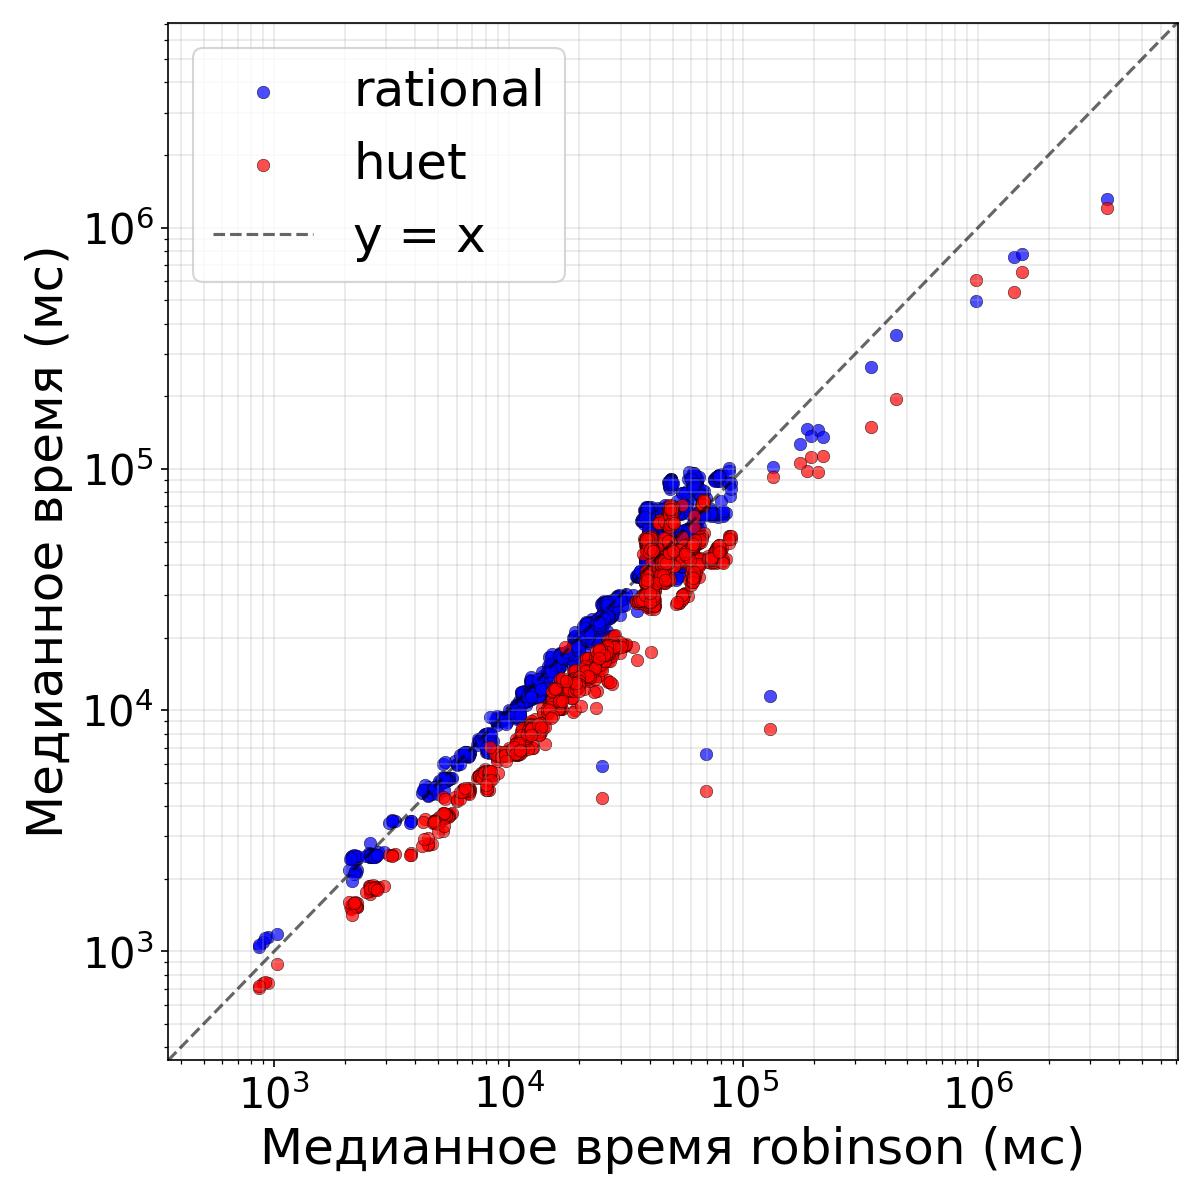
\includegraphics[width=\linewidth]{bench/ephemeral/robinson_comparison.png}
        \subcaption{Эфемерная реализация}
    \end{subfigure}
    \hfill
    \begin{subfigure}{.48\linewidth}
        
\includegraphics[width=\linewidth]{bench/persistent/robinson_comparison.png}
        \subcaption{Персистентная реализация}
    \end{subfigure}
    \caption{Сравнение производительности алгоритмов рациональной унификации по отношению к алгоритму Робинсона.}
    \label{fig:baseline}
\end{figure}

\begin{figure}[b]
    \centering
    \begin{subfigure}{.48\linewidth}
        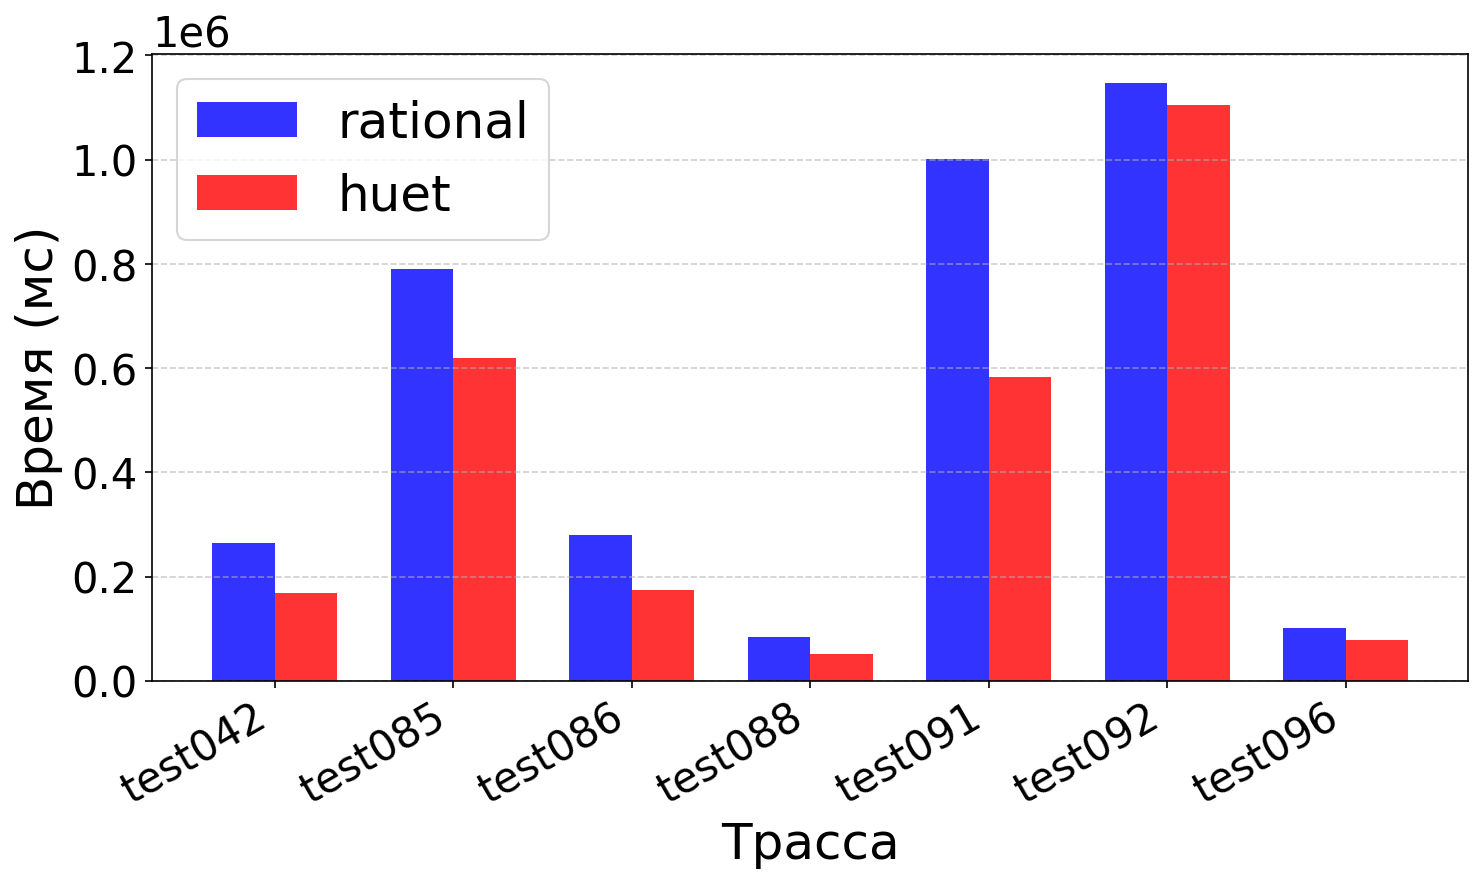
\includegraphics[width=\linewidth]{bench/ephemeral/Lama.png}
        \subcaption{Эфемерная реализация}
    \end{subfigure}
    \hfill
    \begin{subfigure}{.48\linewidth}
        
\includegraphics[width=\linewidth]{bench/persistent/Lama.png}
        \subcaption{Персистентная реализация}
    \end{subfigure}
    \caption{Сравнение алгоритмов на трассах \texttt{Lama}, которые требуют поддержки рациональной унификации}
    \label{fig:Lama}
\end{figure}

\begin{figure}[p]
    \centering
    \begin{subfigure}{.48\linewidth}
        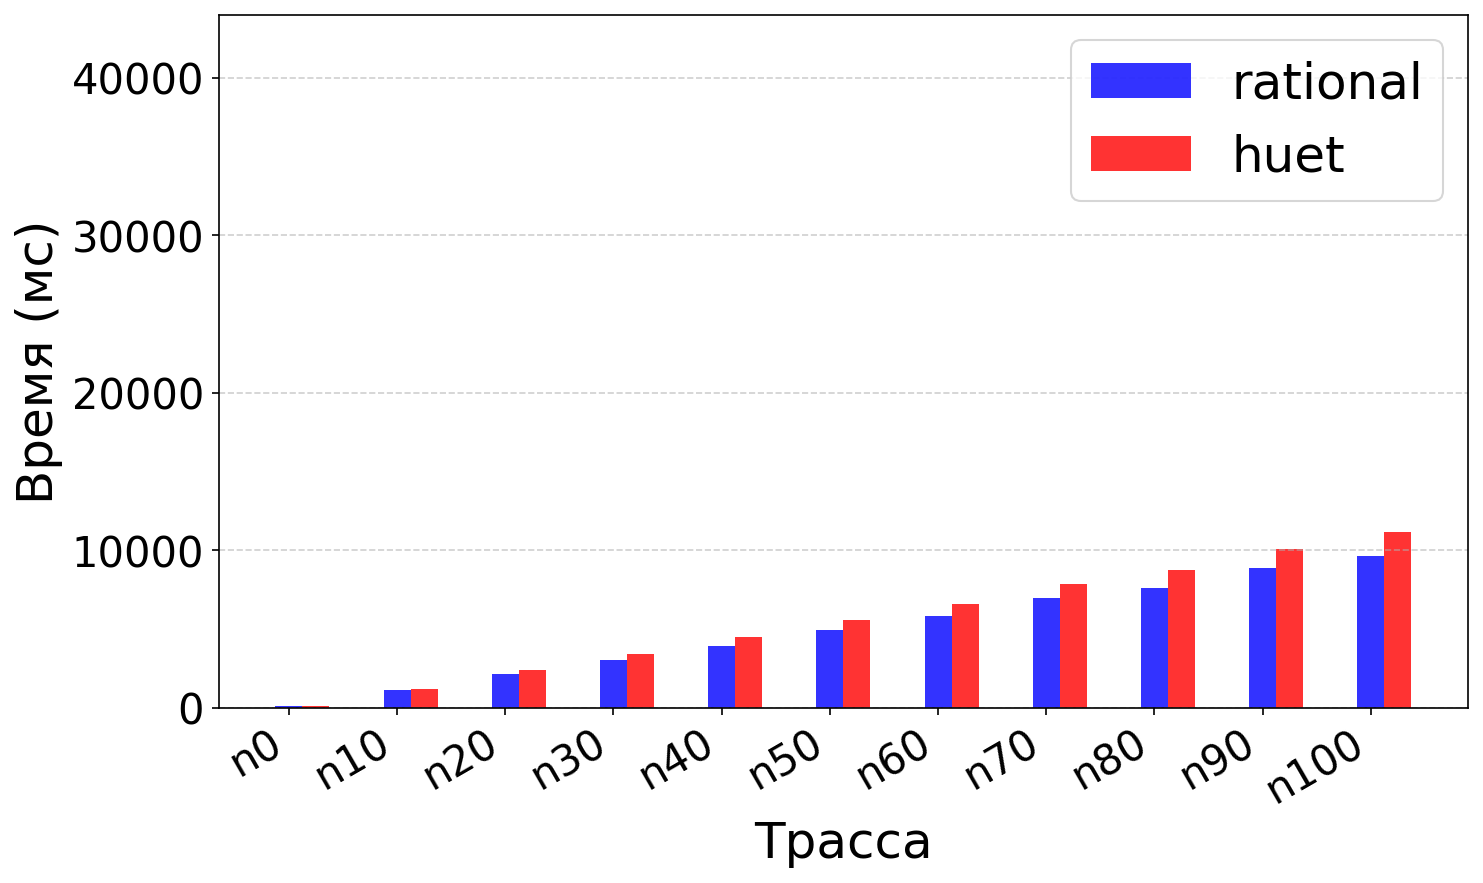
\includegraphics[width=\linewidth]{bench/ephemeral/synth_full.png}
        \subcaption{\texttt{full}}
    \end{subfigure}
    \hfill
    \begin{subfigure}{.48\linewidth}
        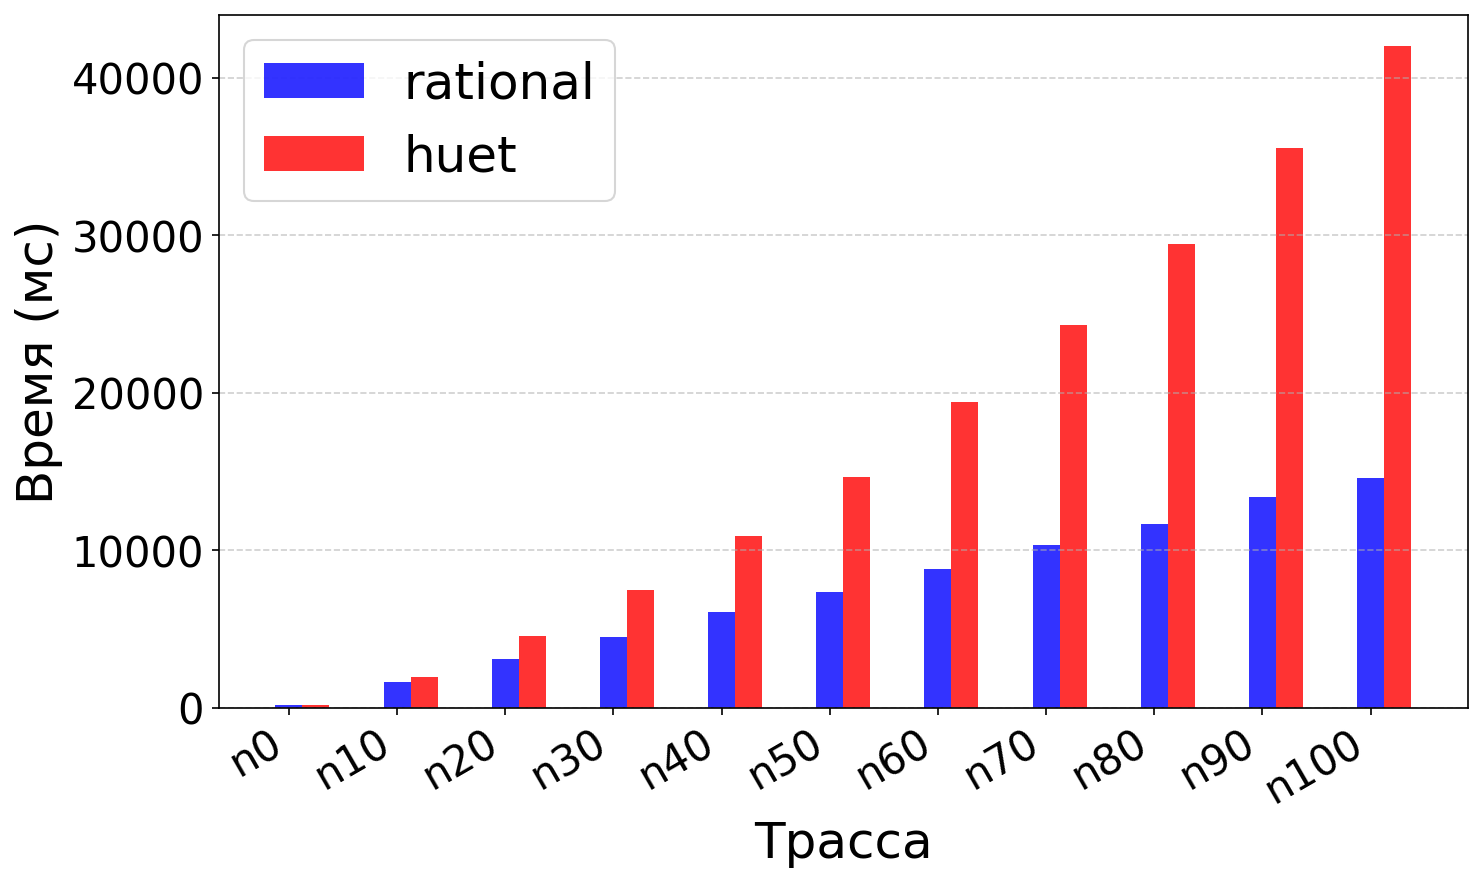
\includegraphics[width=\linewidth]{bench/ephemeral/synth_left_right.png}
        \subcaption{\texttt{left\_right}}
    \end{subfigure}
    \\
    \begin{subfigure}{.48\linewidth}
        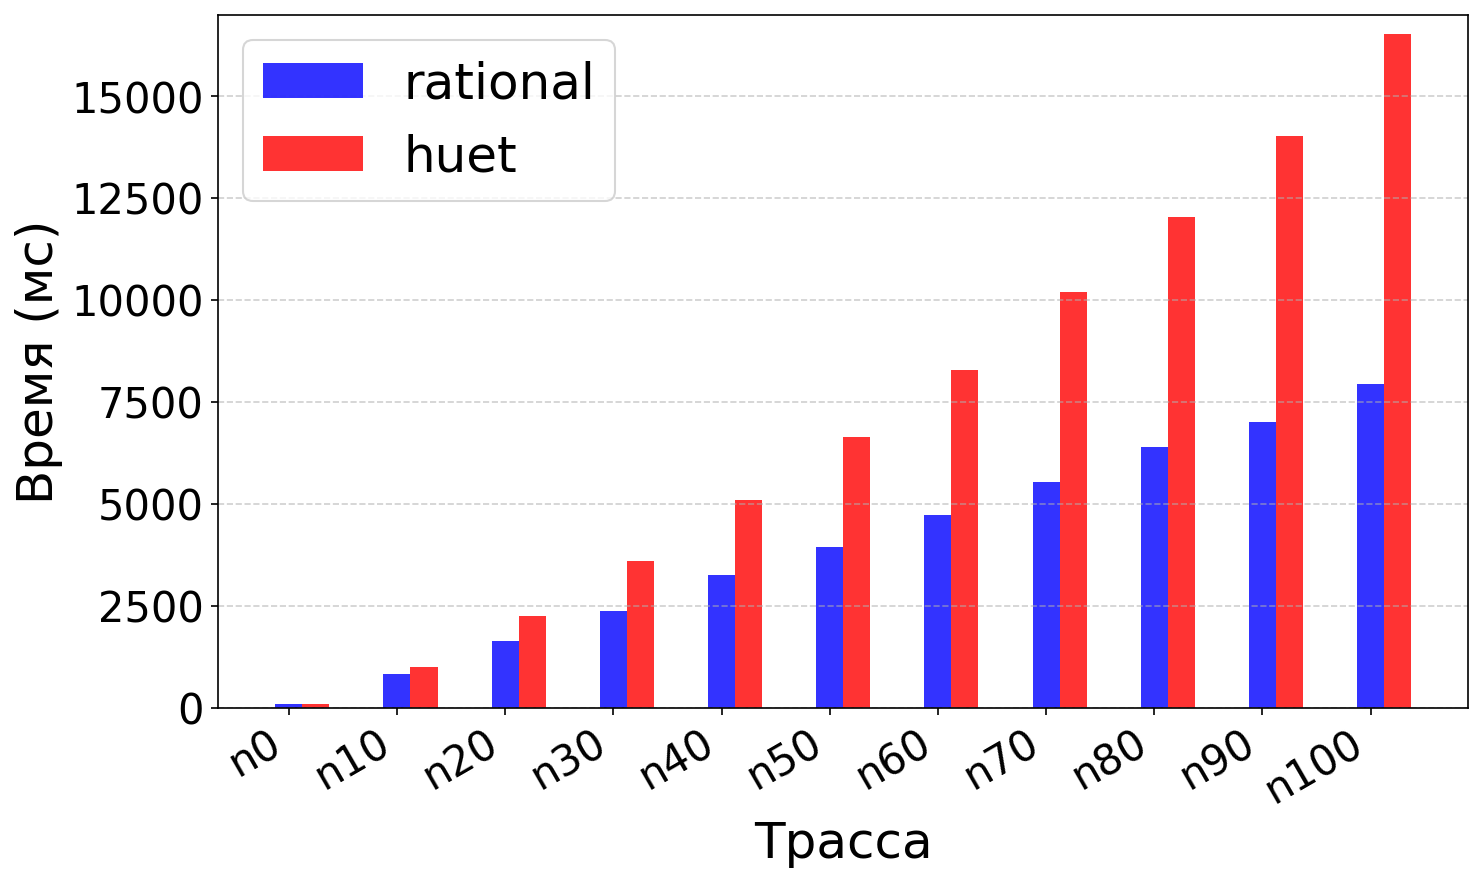
\includegraphics[width=\linewidth]{bench/ephemeral/synth_loops1.png}
        \subcaption{$\texttt{loops}_1$}
    \end{subfigure}
    \hfill
    \begin{subfigure}{.48\linewidth}
        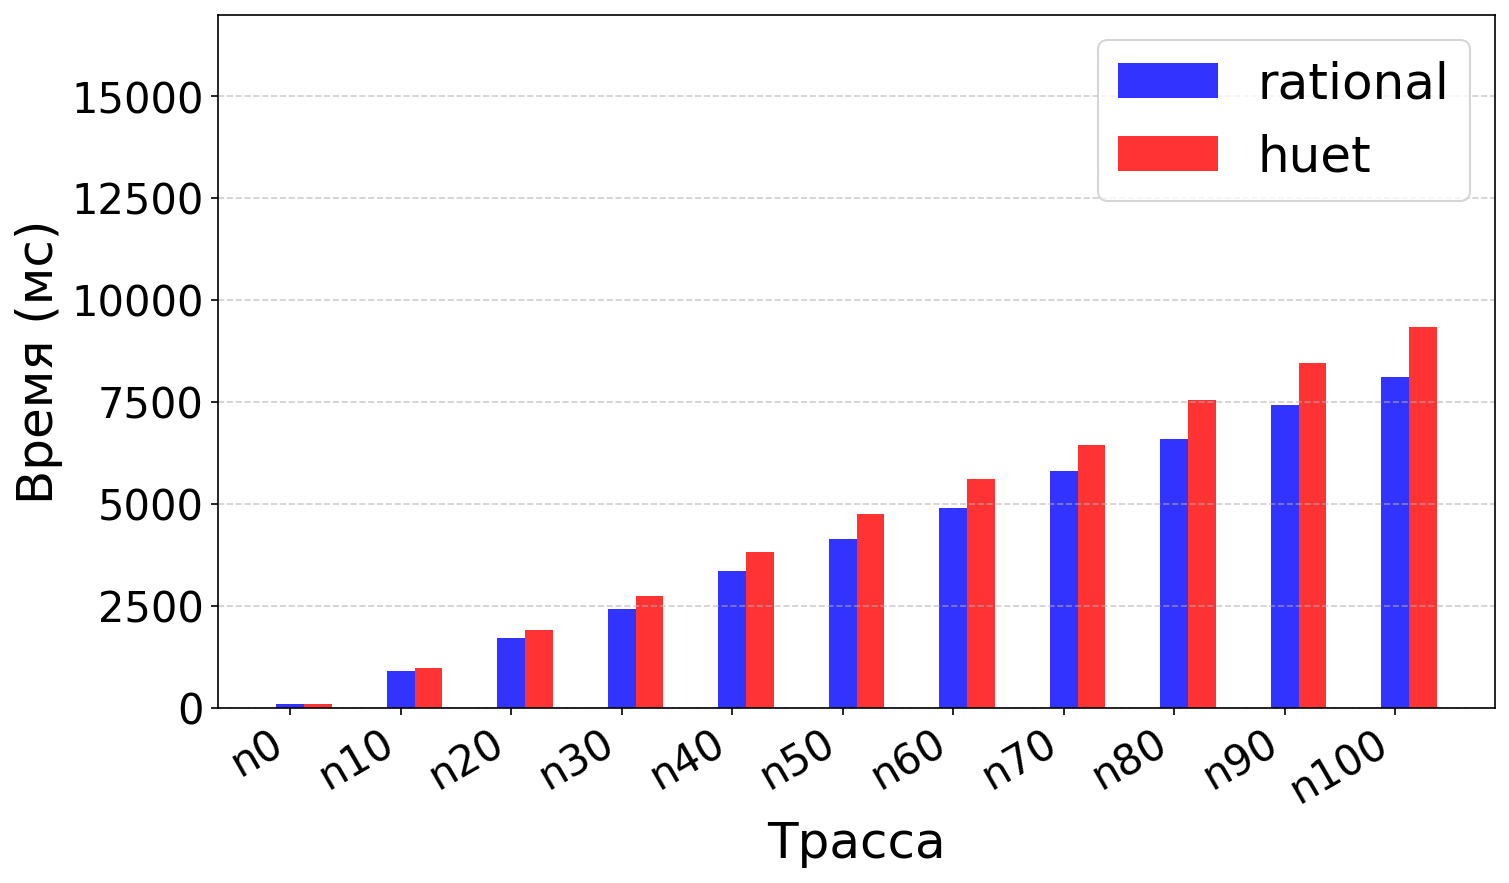
\includegraphics[width=\linewidth]{bench/ephemeral/synth_loops2.png}
        \subcaption{$\texttt{loops}_2$}
    \end{subfigure}
    \\
    \begin{subfigure}{.48\linewidth}
        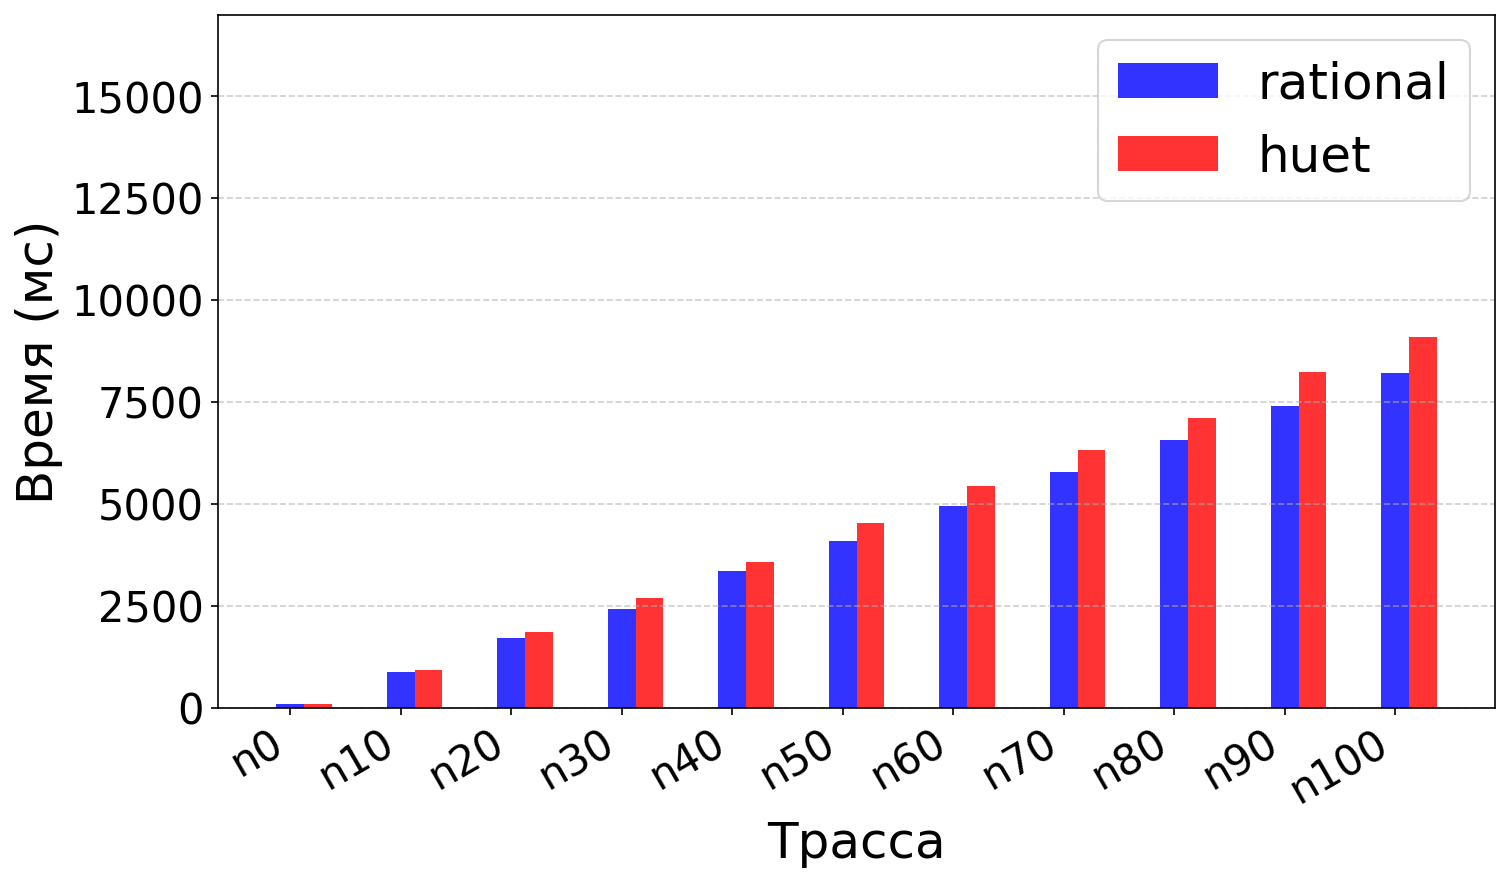
\includegraphics[width=\linewidth]{bench/ephemeral/synth_loops3.png}
        \subcaption{$\texttt{loops}_3$}
    \end{subfigure}
    \hfill
    \begin{subfigure}{.48\linewidth}
        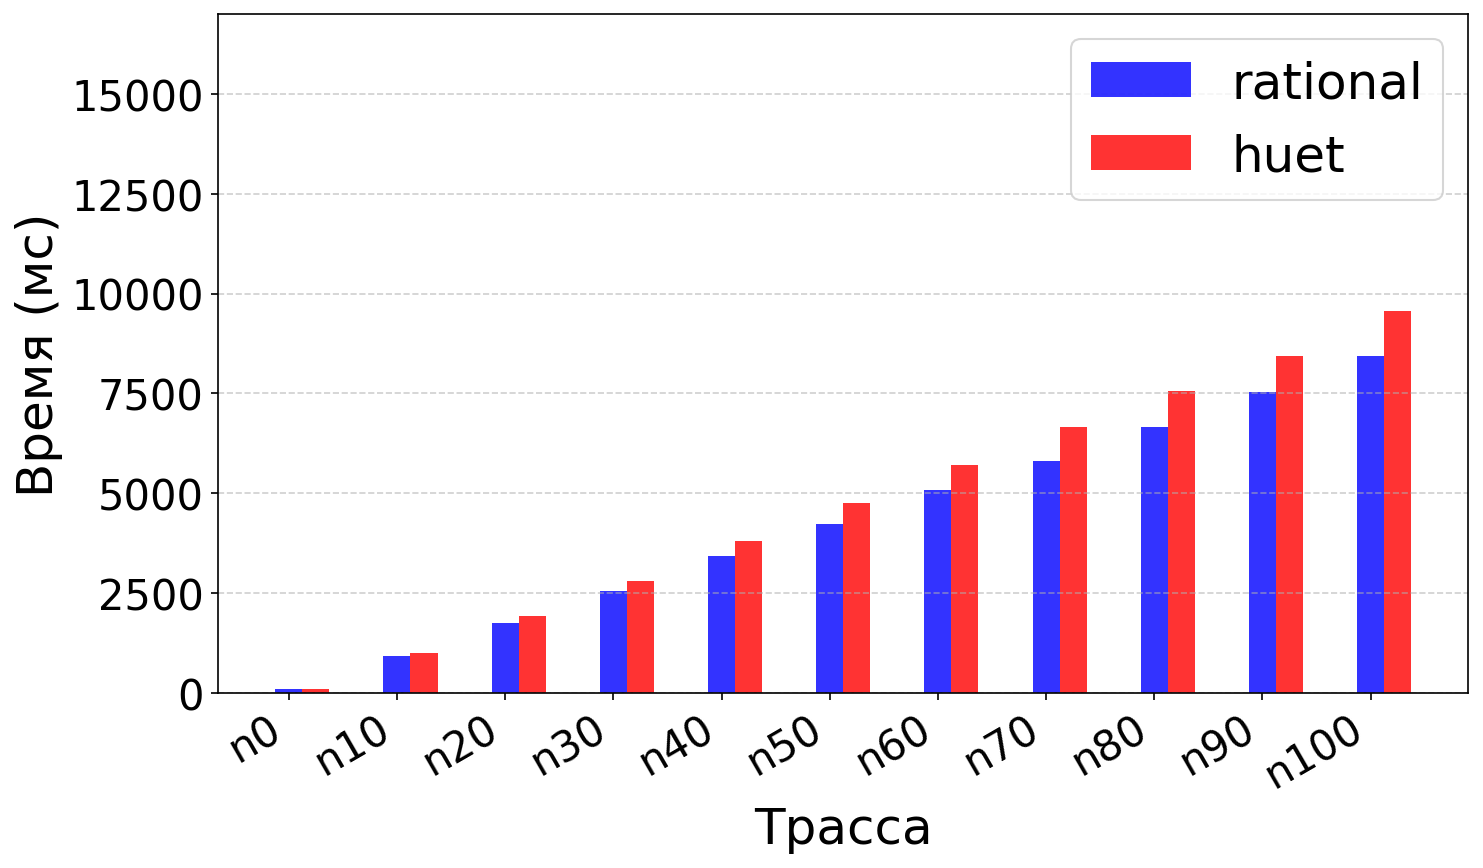
\includegraphics[width=\linewidth]{bench/ephemeral/synth_loops4.png}
        \subcaption{$\texttt{loops}_4$}
    \end{subfigure}
    \caption{Сравнение эфемерных реализаций алгоритмов рациональной унификации на синтетических тестах.}
    \label{fig:synth-ephemeral}
\end{figure}

\begin{figure}[p]
    \centering
    \begin{subfigure}{.48\linewidth}
        
\includegraphics[width=\linewidth]{bench/persistent/synth_full.png}
        \subcaption{\texttt{full}}
    \end{subfigure}
    \hfill
    \begin{subfigure}{.48\linewidth}
        
\includegraphics[width=\linewidth]{bench/persistent/synth_left_right.png}
        \subcaption{\texttt{left\_right}}
    \end{subfigure}
    \\
    \begin{subfigure}{.48\linewidth}
        
\includegraphics[width=\linewidth]{bench/persistent/synth_loops1.png}
        \subcaption{$\texttt{loops}_1$}
    \end{subfigure}
    \hfill
    \begin{subfigure}{.48\linewidth}
        
\includegraphics[width=\linewidth]{bench/persistent/synth_loops2.png}
        \subcaption{$\texttt{loops}_2$}
    \end{subfigure}
    \\
    \begin{subfigure}{.48\linewidth}
        
\includegraphics[width=\linewidth]{bench/persistent/synth_loops3.png}
        \subcaption{$\texttt{loops}_3$}
    \end{subfigure}
    \hfill
    \begin{subfigure}{.48\linewidth}
        
\includegraphics[width=\linewidth]{bench/persistent/synth_loops4.png}
        \subcaption{$\texttt{loops}_4$}
    \end{subfigure}
    \caption{Сравнение персистентных реализаций алгоритмов рациональной унификации на синтетических тестах.}
    \label{fig:synth-persistent}
\end{figure}

Основной причиной такого поведения алгоритма Юэ скорее всего является накопление классов эквивалентности между отдельными экземплярами термов-конструкторов. Теоретическое определение алгоритма предполагает, что всем таким экземплярам присвоен уникальный номер, на основе которого можно строить классы эквивалентности таким же образом, как это делает наш алгоритм с номерами переменных. Тем не менее, на практике такие номера не вводятся из-за дополнительных накладных расходов, а вместо этого они моделируются с помощью дополнительной ячейки памяти внутри объектов, в которые при необходимости записывается ссылка на другой экземпляр.

Естественно, такой подход работает довольно быстро в эфемерном случае, но приводит к увеличению последовательностей разыменования указателей. В то же время, такой подход абсолютно неприменим для персистентной реализации, что вынуждает на самом деле вводить уникальную нумерацию на объектах и поддерживать классы эквивалентности в персистентном хранилище вместе с классами эквивалентности переменных.

Помимо увеличения времени самого разыменования это приводит к увеличению размера персистентного хранилища, что, в свою очередь, замедляет и определение классов эквивалентности переменных. Дополнительным неудобством является то, что ведение нумерации само по себе добавляет накладные расходы и требует более сложной организации хранения термов в памяти.

\begin{table}[h!]
    \centering
    \begin{tabular}{l||c|c|c}
        \toprule
        \bf Алгоритм & \bf Эфемерный & \bf\makecell{Эфемерный со \\ сжатием путей} & \bf Персистентный \\
        \midrule
        Классический & 755 & 915 & \bf 1982 \\
        Наш & 847 & 727 & \bf 2155 \\
        Юэ & \bf 2677 & \bf 2651 & 62 \\
        \bottomrule
    \end{tabular}
    \caption{Число статистически значимых <<побед>> каждого алгоритма в рамках одного варианта реализации на всех трассах.}
    \label{tab:analyse}
\end{table}

Для получения более строгой количественной оценки результатов мы также оценили различия между распределениями времени работы алгоритмов на каждой трассе с помощью критерия Краскела-Уоллиса~\cite{kruskal1952use}. В случае выявления статистически значимых различий выполнялись апостериорные попарные сравнения с использованием критерия Данна~\cite{dunn1964multiple} с поправкой Бонферрони~\cite{bonferroni1936teoria}. В результате для каждой трассы было определено, какой алгоритм имеет статистически значимо меньшее время работы в рамках каждого варианта реализации. Итоговые результаты анализа приведены в \autoref{tab:analyse} в виде числа <<побед>> по каждому алгоритму в рамках одного варианта реализации.

Наконец, мы убедились в том, что сжатие путей не улучшает производительность унификации, что показано в \autoref{tab:analyse-ephemeral}.

\begin{table}[h!]
    \centering
    \begin{tabular}{l||c|c|c}
        \toprule
        \textbf{Вариант} & \textbf{Классический} & \textbf{Наш} & \textbf{Юэ} \\
        \midrule
        Эфемерный & \textbf{597} & \textbf{784} & 494 \\
        Эфемерный со сжатием путей & 470 & 345 & \textbf{685} \\
        \midrule
        Среднее отношение медиан & 1,02 & 1,00 & 1,02 \\
        \bottomrule
    \end{tabular}
    \caption{Число статистически значимых <<побед>> эфемерных вариантов реализации в рамках одного алгоритма на всех трассах.}
    \label{tab:analyse-ephemeral}
\end{table}

